\documentclass[a4paper, 12pt, one column]{article}
\usepackage[utf8]{inputenc}
\usepackage[top = 2.0cm, bottom = 2.0cm, right = 2.0cm, left = 2.0cm, heightrounded, marginparwidth = 1.5cm, marginparsep = 0.4cm, margin = 2.5cm]{geometry}
\usepackage{amsmath}
\usepackage{graphicx}
\graphicspath{{images/}}
\usepackage{float}
\usepackage{subcaption}
\usepackage{indentfirst}
\usepackage{siunitx}
\usepackage{amsmath}
\usepackage{listings}
\usepackage{color}
\usepackage{booktabs}
\usepackage[backend=bibtex,style=authoryear]{biblatex}
\addbibresource{references.bib}

% Define colors for listings
\definecolor{codegreen}{rgb}{0.0, 0.5, 0.26}  % A softer green
\definecolor{codegray}{rgb}{0.4, 0.4, 0.4}   % A darker gray for better contrast
\definecolor{codepurple}{rgb}{0.7, 0.0, 0.5} % A muted purple
\definecolor{backcolour}{rgb}{0.98, 0.98, 0.98} % A very light gray background


% Define the style for listings
\lstdefinestyle{mystyle}{
    backgroundcolor=\color{backcolour},   
    commentstyle=\color{codegreen},
    keywordstyle=\color{magenta},
    numberstyle=\tiny\color{codegray},
    stringstyle=\color{codepurple},
    basicstyle=\ttfamily\footnotesize,
    breakatwhitespace=false,         
    breaklines=true,                 
    captionpos=b,                    
    keepspaces=true,                 
    numbers=left,                    
    numbersep=5pt,                  
    showspaces=false,                
    showstringspaces=false,
    showtabs=false,                  
    tabsize=2
}
\lstset{style=mystyle}


\title{QBS 103 Final Submission}

\author{Haoyang Cui}
\date{Aug. 29th, 2 p.m.}

\begin{document}


\maketitle

\section{Data Select}
We pick up the data from arge-Scale Multi-omic Analysis of COVID-19
Severit, \cite{Overmyer2021}\\
For the data we use, we delete the participant \_id NONCOVID\_15\_83y\_unknown\_ICU as we can not access its sex data, so we give up this one. And there is a wrong participant\_id, I use setdiff function to find it and make the two id same. We use the tidyverse package, \cite{tidyverse_2023} to edit the data.\\
\begin{lstlisting}[language=Python]
genes <- read.csv("QBS103_GSE157103_genes.csv")
matrix <- read.csv("QBS103_GSE157103_series_matrix.csv")

id_genes <- colnames(genes)
id_genes <- id_genes[-1]
id_matrix <- matrix$participant_id
diff1 <- setdiff(id_genes, id_matrix)
diff2 <- setdiff(id_matrix, id_genes)
colnames(genes)[colnames(genes) == diff1] <- diff2
matrix <- matrix %>% rename('procalcitonin.ng.ml.' = 'procalcitonin.ng.ml..')

unknown_id <- matrix$'participant_id'[matrix$sex == ' unknown']

matrix <- matrix[!matrix$participant_id %in% unknown_id, ]
genes[[unknown_id]] <- NULL
\end{lstlisting}
\section{Table}
\subsection{Variable Choose}
For the table, we generate 3 category variable: sex, disease\_status and icu\_status, and 3 continuous variable: age, ferritin and procalcitonin.

\subsection{Table}
\begin{table}[h!]
\centering
\caption*{Comparison of COVID-19 and non-COVID-19 patients}
\begin{tabular}{lccc}
\toprule
& \textbf{Male} & \textbf{Female} & \textbf{Overall} \\
 & \textbf{(N=74)} & \textbf{(N=51)} & \textbf{(N=125)} \\
\textbf{Category} & & &\\
\midrule
 \textbf{Disease Status} & & &\\
\midrule
COVID-19 & 62 (83.8\%)& 38 (74.5\%) & 100 (80\%) \\
non-COVID-19 & 12 (16.2\%)& 13 (25.5\%) & 25 (20\%) \\
\midrule
\textbf{Icu Status} & & & \\
Yes& 41(55.4\%)& 24 (47.1\%)& 65(52\%)\\
No& 33(44.6\%)& 27(52.9\%)& 60(48.0\%)\\
\midrule
\textbf{Continuous} & & &\\
\midrule
\textbf{Age} & & & \\
Mean (SD) & 62.3 (14.4) & 59.3 (18.0) & 61.1 (15.9) \\
Median [Min, Max] & 63 [27, 88] & 62 [21, 86] & 62.0 [21.0, 88.0] \\
\midrule
\textbf{ferritin.ng.ml.} & & & \\
Mean (SD) & 993.3 (1013.0)& 619.3 (1054.3)& 833.5 (1042.8)\\
Median [Min, Max] & 755 [58, 5971]& 318 [14, 5508]& 573 [14, 5971]\\
\midrule
\textbf{procalcitonin.ng.ml.} & & & \\
Mean (SD) & 2.47 (5.79)& 3.94 (13.65)& 3.08 (9.79)\\
Median [Min, Max] & 0.69 [0.05, 36.00]& 0.500 [0.05, 86.39]& 0.5 [0.05, 86.39]\\
\bottomrule
\end{tabular}
\end{table}
From the table, Male patients were slightly higher than female patients in terms of COVID-19 infection rate, proportion of admission to ICU, and ferritin levels, while female patients had significantly higher procalcitonin levels than male patients.
\newpage

\section{New plot type}
To introduce more about the category relation, I use the faceting barplot named facet\_grid in ggplot2 (\cite{ggplot2_2024}), and add count number on it by using geom\_text.

\begin{lstlisting}[language=Python]
selected_table %>%
  ggplot(aes(x = sex, fill = disease_status)) +
  geom_bar() +
  facet_grid(icu_status ~ .) +
  geom_text(aes(label = ..count..), stat = "count", position = position_stack(vjust = 0.5)) +
  scale_fill_manual(values = c("disease state: COVID-19" = "#f69F00", "disease state: non-COVID-19" = "#5654E9")) +
  labs(x = "sex", fill = "disease_status", title = "Occupation by ICU Status, Sex, and Disease Status") +
  theme_minimal()
\end{lstlisting}

\begin{figure}[H]
    \centering
    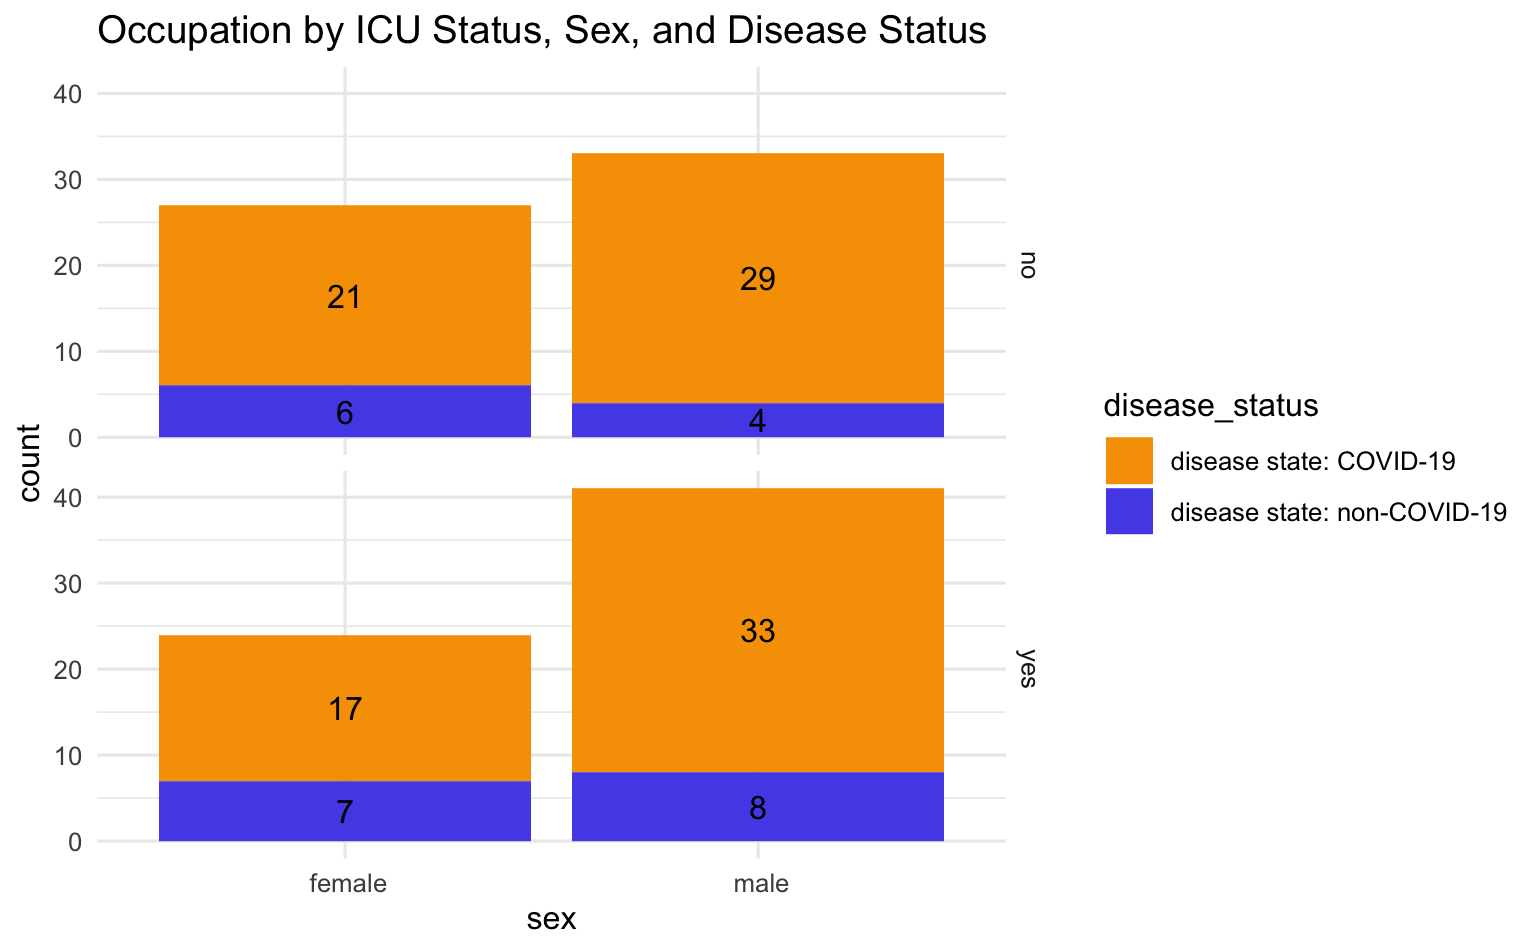
\includegraphics[width=1\textwidth]{new_map.png} 
    \caption{Bar plot with faceting}
    \label{faceting}
\end{figure}
From figure \ref{faceting}, the COVID-19 infection rate in male patients was slightly higher than that in female patients, regardless of whether they were admitted to the ICU. And among all patients, the number of people with Covid-19 was much higher than that of non-COVID patients.

\section{Histogram, Scatter plot, and Boxplot from submission 1}
We still use the ggplot2 (\cite{ggplot2_2024}) to observe the gene AAMP.

\begin{figure}[H]
    \centering
    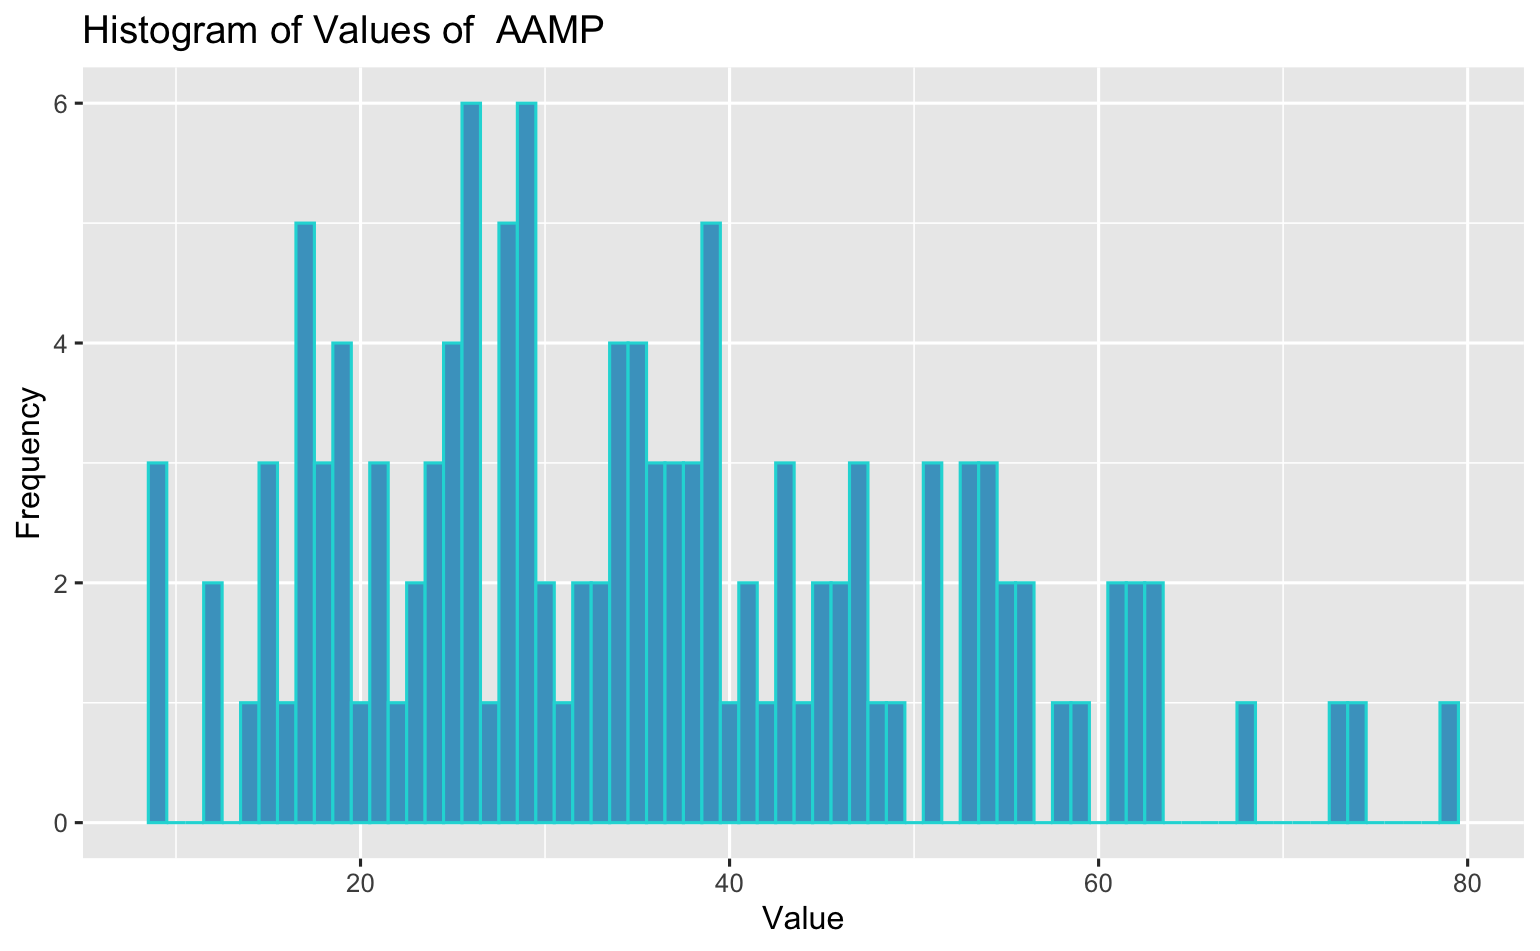
\includegraphics[width=1\textwidth]{hist.png}
    \caption{Histogram for AAMP}
    \label{hist}
\end{figure}
From figure \ref{hist}, the gene value of AAMP has a relatively uniform distribution in different intervals, with the highest frequency appearing between about 20 and 40. The gene values in these intervals appear more frequently, with 5 to 6 occurrences in each interval. It shows a relatively dispersed distribution pattern with no obvious central trend.

\begin{figure}[H]
    \centering
    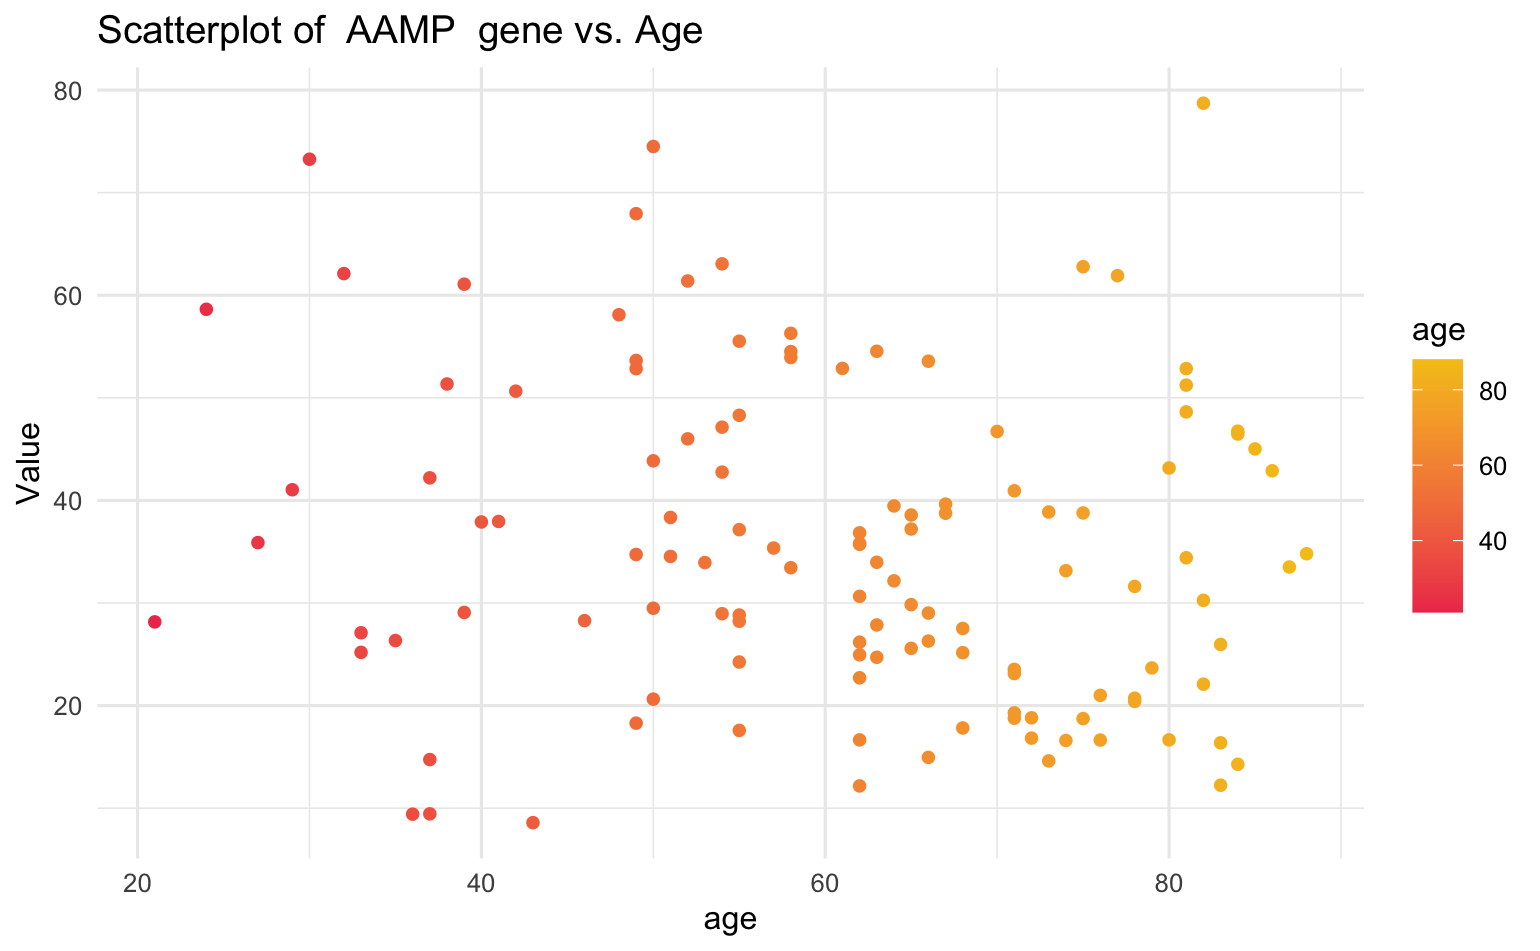
\includegraphics[width=1\textwidth]{scatter.png} 
    \caption{Scatterplot for AAMP}
    \label{scatter}
\end{figure}
From figure \ref{scatter}, AAMP gene values were distributed across age groups, but there was no obvious linear trend, indicating that there may not be a direct correlation between AAMP values and age.\\
However, we can observe that there is a certain clustering of AAMP gene values in the middle-aged group, especially in areas with lower gene values.

\begin{figure}[H]
    \centering
    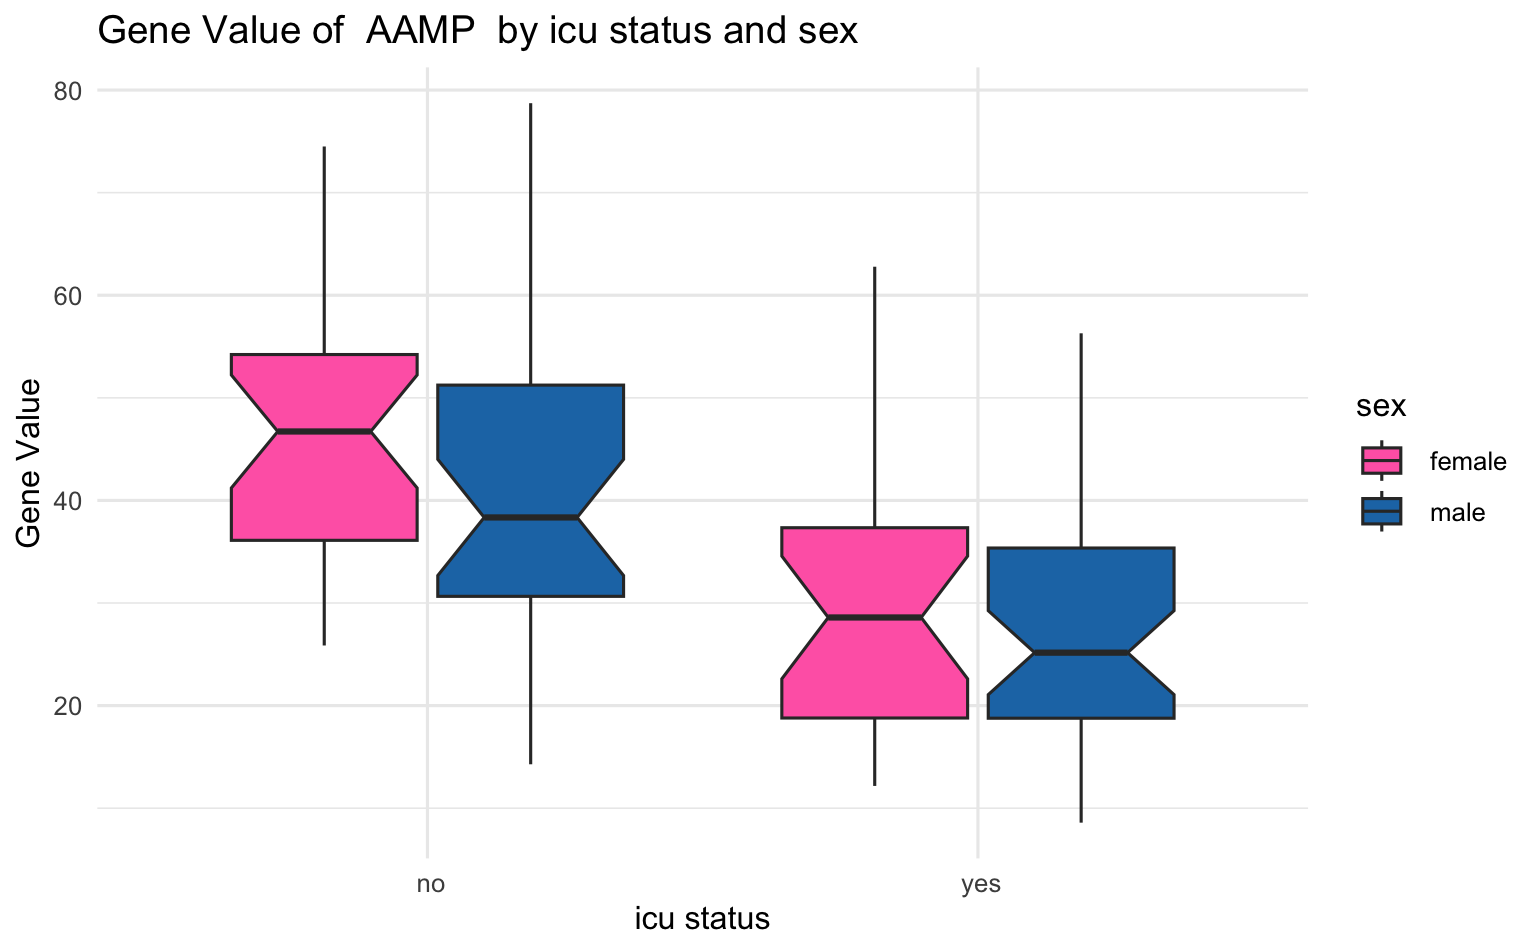
\includegraphics[width=1\textwidth]{box_plot.png}     
    \caption{Boxplot for AAMP}
    \label{Box}
\end{figure}
From figure \ref{Box}, there was no significant difference in the gene values between the sexes. The median gene values for patients admitted to the ICU tended to be slightly lower.


\section{Heatmap}

To build the heatmap, we use the package pheatmap (\cite{pheatmap}), labeled the icu\_status and sex as annotation.
\begin{figure}[H]
    \centering
    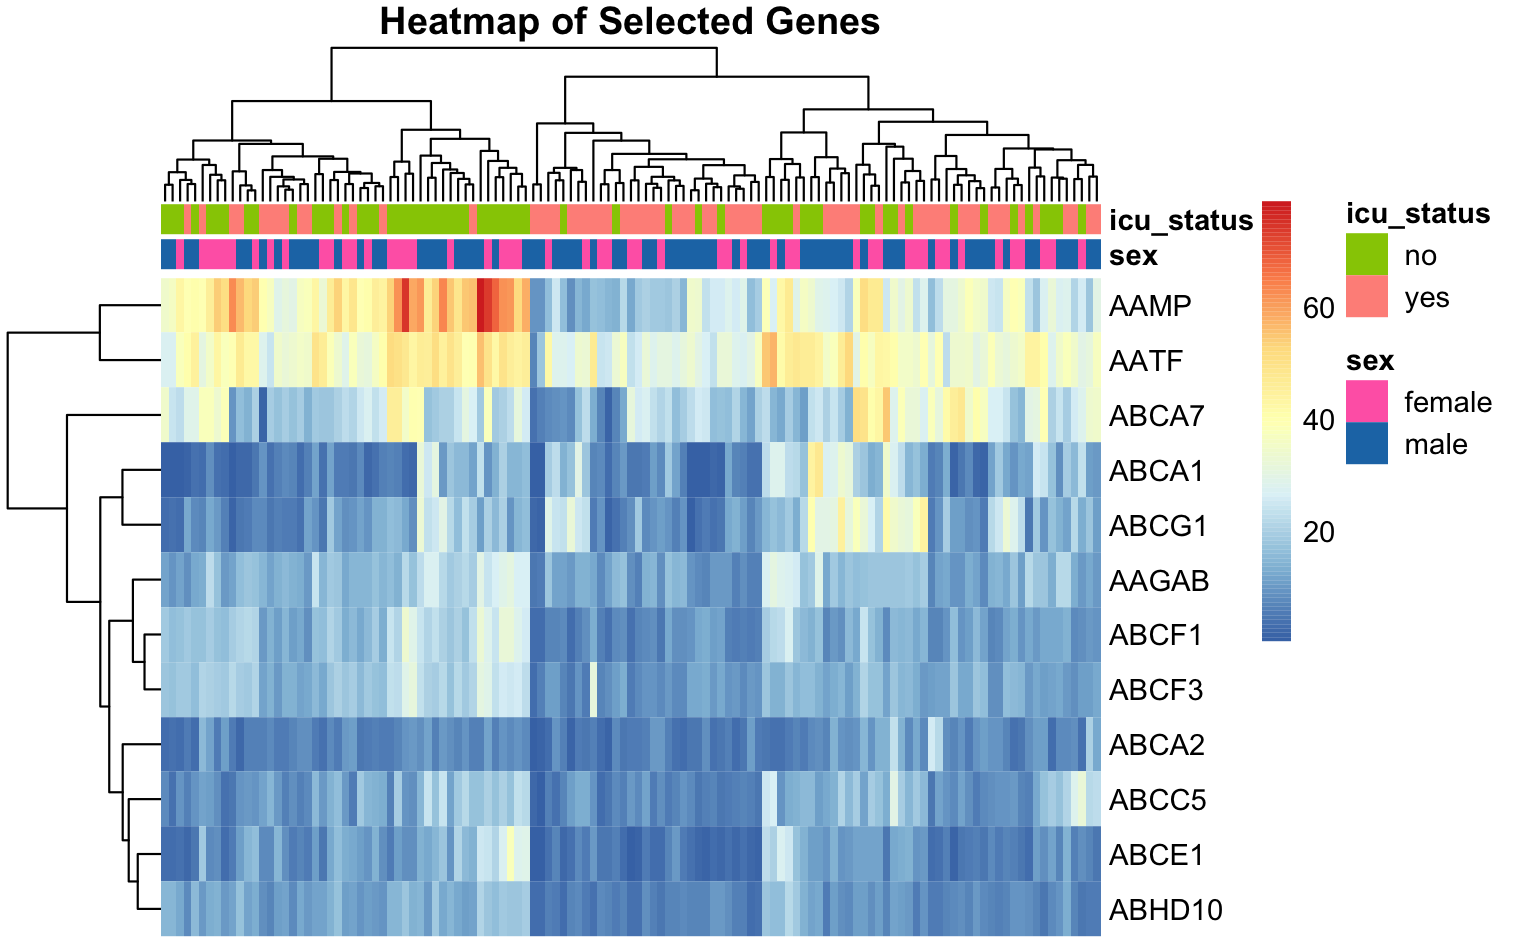
\includegraphics[width=1\textwidth]{heatmap.png} 
    \caption{Heatmap}
    \label{heat}
\end{figure}
The results of figure \ref{heat} show that gene expression varies greatly among different individuals, especially in gene regions with high gene values.


\printbibliography
\end{document}
